\documentclass[11pt,a4paper]{report}

% Paquetes necesarios

% Configuración de fuente Arial 11pt
% Para usar Arial real, compila con XeLaTeX en lugar de pdfLaTeX
\usepackage{fontspec}
\setmainfont{Arial}

\newfontfamily\bellmt{Bell MT}[
  ItalicFont = {Bell MT Italic},
]

\usepackage[spanish,es-tabla]{babel}
\usepackage[margin=2.54cm]{geometry} % Márgenes de 2.54cm
\usepackage{setspace} % Control de interlineado
\usepackage{graphicx} % Para incluir imágenes
\usepackage{fancyhdr} % Para encabezados y pies de página
\usepackage{titlesec} % Para formato de títulos
\usepackage{tocloft} % Para personalizar índices
\usepackage{indentfirst} % Sangría en primer párrafo
\usepackage{hyperref} % Enlaces en el PDF
\usepackage{float} % Para posicionamiento de figuras
\usepackage{caption} % Para personalizar captions
\usepackage{subcaption} % Para subfiguras
\usepackage{array} % Para tablas
\usepackage{booktabs} % Para tablas profesionales
\usepackage{multirow} % Para celdas multirow en tablas
\usepackage{amsmath} % Para matemáticas
\usepackage{csquotes} % Para citas
\usepackage[style=apa,backend=biber]{biblatex} % Para bibliografía APA 7
\usepackage{appendix} % Para apéndices

% Configuración de bibliografía
\addbibresource{references.bib}

% Configuración de interlineado
\doublespacing % Interlineado doble

% Configuración de sangría
\setlength{\parindent}{1.27cm} % Sangría de primera línea

% Configuración de espaciado entre párrafos
\setlength{\parskip}{0pt} % Sin espacio extra entre párrafos

% Configuración de numeración de páginas
\pagestyle{fancy}
\fancyhf{}
\fancyhead[R]{\thepage} % Número de página en esquina superior derecha
\renewcommand{\headrulewidth}{0pt} % Sin línea en encabezado

% Configuración de formato de títulos según FORMAT.md
% Nivel 1: Bold, 14-18pt, UPPERCASE, centrado, sin numeración
\titleformat{\chapter}[display]
{\normalfont\bfseries\centering\fontsize{16}{19.2}\selectfont}{}{0pt}{\MakeUppercase}
\titlespacing*{\chapter}{0pt}{-30pt}{20pt}

% Nivel 2: Bold, 11pt, izquierda, sin numeración
\titleformat{\section}
{\normalfont\bfseries\raggedright}{}{0pt}{}
\titlespacing*{\section}{0pt}{0pt}{0pt}

% Nivel 3: Bold Italic, 11pt, izquierda, sin numeración
\titleformat{\subsection}
{\normalfont\bfseries\itshape\raggedright}{}{0pt}{}
\titlespacing*{\subsection}{0pt}{0pt}{0pt}

% Nivel 4: Bold, sangría 1.27cm, inline con punto
\titleformat{\subsubsection}[runin]
{\normalfont\bfseries}{}{0pt}{}[.]
\titlespacing*{\subsubsection}{\parindent}{0pt}{1em}

% Nivel 5: Bold Italic, sangría 1.27cm, inline con punto
\titleformat{\paragraph}[runin]
{\normalfont\bfseries\itshape}{}{0pt}{}[.]
\titlespacing*{\paragraph}{\parindent}{0pt}{1em}

% Configuración de captions para tablas y figuras (Arial 10pt exacto)
\DeclareCaptionFont{arial10}{\fontsize{10}{12}\selectfont}
\captionsetup{
    font={arial10,doublespacing},
    labelfont=bf,
    textfont=it,
    justification=centering,
    singlelinecheck=false
}

% Configuración de índices
\renewcommand{\contentsname}{Índice de contenido}
\renewcommand{\listtablename}{Índice de tablas}
\renewcommand{\listfigurename}{Índice de figuras}

% Comando para páginas sin numeración pero contadas
\newcommand{\unnumberedpage}{%
    \thispagestyle{empty}
    \addtocounter{page}{1}
}

% Comando para eliminar sangría (para secciones preliminares)
\newcommand{\noindentpages}{%
    \setlength{\parindent}{0pt}
}

% Comando para restaurar sangría (desde Introducción)
\newcommand{\restoreindent}{%
    \setlength{\parindent}{1.27cm}
}

% Documento principal
\begin{document}

% Páginas preliminares con números romanos (sin sangría)
\pagenumbering{roman}
\setcounter{page}{1}
\noindentpages

% Carátula (sin numerar pero contada)
\unnumberedpage
\begin{center}
    
    
\includegraphics[width=3.5cm]{figures/logo_utpl.jpg} % Asegúrate de tener el logo
    
    \vspace{1cm}
    
    {\Large \textbf{UNIVERSIDAD TÉCNICA PARTICULAR DE LOJA}}\\
    {\large \textit{La Universidad Católica de Loja}}
    
    \vspace{1cm}
    
    {\large \textbf{FACULTAD DE XXXXXXX}}
    
    \vspace{1cm}
    
    {\large \textbf{MAESTRÍA EN XXXXXXXX}}
    
    \vspace{1cm}
    
    {\Large \textbf{Xxxxx xxxx xxxxxx xxxx}}
    
    \vspace{1cm}
    
    {\large Trabajo de titulación previo a la obtención del título de:}
    
    \vspace{1cm}
    
    {\large \textbf{XXXXXXX XXXXXXX}}
    
    \vspace{2cm}
    
    \begin{flushleft}
    \hspace{3cm}{\large \textbf{Autor:} Apellido1 Apellido2, Nombre1 Nombre2}\\
    \vspace{0.5cm}
    \hspace{3cm}{\large \textbf{Director:} Apellido1 Apellido2, Nombre1 Nombre2}
    \end{flushleft}
    
    \vfill
    
    {\large LOJA}\\
    {\large 2025}
    
    \end{center}
\clearpage

% Aprobación del director
\chapter*{Aprobación del director del Trabajo de Titulación}
\addcontentsline{toc}{chapter}{Aprobación del director del Trabajo de Titulación}

\vspace{1cm}

Loja, día de mes de año

\vspace{1cm}

Título académico completo, (no colocar siglas)\\
Nombres y Apellidos completos del director de la carrera\\
\textbf{Director de la maestría de Xxxxxxxxxx}\\
Ciudad.-

\vspace{1cm}

De mi consideración:

\vspace{0.5cm}

Me permito comunicar que, en calidad de director del presente Trabajo de Titulación nominado: (nombre del trabajo) realizado por Nombres y Apellidos completos del autor o autores (as) ha sido orientado y revisado durante su ejecución, así mismo ha sido verificado a través de la herramienta de similitud académica institucional, y cuenta con un porcentaje de coincidencia aceptable. En virtud de ello, y por considerar que el mismo cumple con todos los parámetros establecidos por la Universidad, doy mi aprobación a fin de continuar con el proceso académico correspondiente.

\vspace{0.5cm}

Particular que comunico para los fines pertinentes.

\vspace{1cm}

Atentamente,

\vspace{3cm}

\noindent
\rule{8cm}{0.4pt}\\
Director: Nombres y Apellidos completos del Director del Trabajo de Titulación y título académico.\\
C.I.:\\
Correo electrónico:
\clearpage

% Declaración de autoría
\chapter*{Declaración de autoría y cesión de derechos}
\addcontentsline{toc}{chapter}{Declaración de autoría y cesión de derechos}

Yo, Luis Antonio Pillaga Zhagñay, declaro y acepto en forma expresa lo siguiente:

Ser autor del Trabajo de Titulación denominado: Desarrollo de un prototipo móvil para la lectura de medidores de agua potable usando técnicas de procesamiento de imágenes, de la maestría en Inteligencia Artificial Aplicada, específicamente de los contenidos comprendidos en: Introducción, Capítulo 1: Marco Teórico, Capítulo 2: Metodología, Capítulo 3: Desarrollo y Resultados, Conclusiones y Recomendaciones, siendo Guido Eduardo Riofrio Calderón, director del presente trabajo; también declaro que la presente investigación no vulnera derechos de terceros ni utiliza fraudulentamente obras preexistentes. Además, ratifico que las ideas, criterios, opiniones, procedimientos y resultados vertidos en el presente trabajo investigativo, son de mi exclusiva responsabilidad. Eximo expresamente a la Universidad Técnica Particular de Loja y a sus representantes legales de posibles reclamos o acciones judiciales o administrativas, en relación a la propiedad intelectual de este trabajo.

Que la presente obra, producto de mis actividades académicas y de investigación, forma parte del patrimonio de la Universidad Técnica Particular de Loja, de conformidad con el artículo 20, literal j), de la Ley Orgánica de Educación Superior; y, artículo 91 del Estatuto Orgánico de la UTPL, que establece: ``Forman parte del patrimonio de la Universidad la propiedad intelectual de investigaciones, trabajos científicos o técnicos y tesis de grado que se realicen a través, o con el apoyo financiero, académico o institucional (operativo) de la Universidad'', en tal virtud, cedo a favor de la Universidad Técnica Particular de Loja la titularidad de los derechos patrimoniales que me corresponden en calidad de autor/a, de forma incondicional, completa, exclusiva y por todo el tiempo de su vigencia.

La Universidad Técnica Particular de Loja queda facultada para ingresar el presente trabajo al Sistema Nacional de Información de la Educación Superior del Ecuador para su difusión pública, en cumplimiento del artículo 144 de la Ley Orgánica de Educación Superior.

\vspace{2.5cm}

\noindent
Autor: Luis Antonio Pillaga Zhagñay\\
C.I.: 0301971495\\
Correo electrónico: lapillaga2@utpl.edu.ec
\clearpage

% Dedicatoria
\chapter*{Dedicatoria}
\addcontentsline{toc}{chapter}{Dedicatoria}

\vspace{2cm}

Xxxxxxxx xxxxxxxx xxxxxxxx xxxxxxxxxxxxxx xxxxxxx xxxxxxx xxxxxx xxxxxx xxxxxxxx xxxxxxxxxx xxxxxxxx xxxxxxxx xxxxxxxxx xxxxxxxxxxxxxxx xxxxxxx xxxxxxxxx.

Xxxxxxxx xxxxxxx xxxxxxxx xxxxxxx xxxxxxxx xxxxxxxxx xxxxxx xxxxx xxxxx xxxxxxxxxx xxxxxxx xxxxxxxxx xxxxxxx xxxxx xxxxxxxx.

Xxxxxxxx xxxxxxx xxxxxxxx xxxxxxx xxxxxxxx xxxxxxxxx xxxxxx xxxxx xxxxx xxxxxxxxxx xxxxxxx xxxxxxxxxxxxxx.
\clearpage

% Agradecimiento
% agradecimiento.tex
\chapter*{Agradecimiento}
\addcontentsline{toc}{chapter}{Agradecimiento}

TODO
\clearpage

% Índice de contenido
\tableofcontents
\clearpage

% Índice de tablas
\listoftables
\clearpage

% Índice de figuras
\listoffigures
\clearpage

% Cambio a números arábigos desde el resumen (sin sangría aún)
\pagenumbering{arabic}
\setcounter{page}{1}

% Resumen
% resumen.tex
\chapter*{Resumen}
\addcontentsline{toc}{chapter}{Resumen}

El resumen se presentará en un único párrafo con un máximo de \textbf{180 palabras}, sintetiza el aporte que brinda el trabajo realizado. \textbf{Obligatoriamente} debe contener las palabras clave \textbf{(máximo tres)}.

\vspace{0.5cm}

Ejemplo:

\vspace{0.5cm}

Xxxxxxxx xxxxxxxx xxxxxxxx xxxxxxxxxxxxxx xxxxxxx xxxxxxx xxxxxx xxxxxx xxxxxxxx xxxxxxxxxx xxxxxxxx xxxxxxxx xxxxxxxxx xxxxxxxxxxxxxxx xxxxxxx xxxxxxxxx xxxxxxx xxxxxxx xxxxxxxx xxxxxxx xxxxxxxx xxxxxxxxx xxxxxx xxxxx xxxxx xxxxxxxxxx xxxxxxx xxxxxxxxxx xxxxxxx xxxxxxxxxx xxxxxxxxx. Xxxxxxxx xxxxxxxx xxxxxxxx xxxxxxxxxxxxxx xxxxxxx xxxxxxx xxxxxx xxxxxx xxxxxxxxxxxxxxxxxxxxx xxxxxxxxxx xxxxxxxx xxxxxxxx xxxxxxxxx xxxxxxxxxxxxxxx xxxxxxx xxxxxxxxxxxxxxxx xxxxxxx xxxxxxxx xxxxxxx xxxxxxxx xxxxxxxxx xxxxxx xxxxx xxxxx xxxxxxxxxx xxxxxxx xxxxxxxxxx xxxxxxx xxxxxx xxxxx xxxxxxx xxxxxx xxxxxxxxxxxxxxxxxxx. Xxxxxxxx xxxxxxxxxxxx xxxxxxxxxxxxx xxxxxxxxxxxxxx xxxxxxx xxxxxxx xxxxxx xxxxxx xxxxxxxxxxxxxxx xxxxxxxxxxxxxxxx xxxxxxxx xxxxxxxx xxxxxxxxx xxxxxxxxxxxxxxx xxxxxxx xxxxxxxxxxxxxxxx xxxxxxx xxxxxxxx xxxxxxx xxxxxxxx xxxxxxxxx xxxxxx xxxxx xxxxx xxxxxxxxxx xxxxxxx xxxxxxxxxx xxxxxxxxxxxxxxxxxxxxxxx xxxxxxxxxxxxx xxxxxxxxxxxxxxxx. Xxxxxxxx xxxxxxxx xxxxxxxx xxxxxxxxxxxxxx xxxxxxx xxxxxxx xxxxxx xxxxxx xxxxxxxxxxxxxxxxxx xxxxxxxxxxxxxxxxxxxx xxxxxxxx xxxxxxxx xxxxxxxxx xxxxxxxxxxxxxxx xxxxxxx xxxxxxxxxxxxxxxx xxxxxxx xxxxxxxx xxxxxxx xxxxxxxx xxxxxxxxx xxxxxx xxxxx xxxxx xxxxxxxxxx xxxxxxx xxxxxxxxxx xx xxxxx xxxxxxx xxxxxx xxxxxxxxxxxxxxxx xxxxxxxxxxxxxx.

\vspace{0.5cm}

\textbf{\textit{Palabras clave:}} xxxxxxxxx, xxxxxxxx, xxxxxx.
\clearpage

% Abstract
\chapter*{Abstract}
\addcontentsline{toc}{chapter}{Abstract}

Abstract es el resumen traducido al idioma inglés en donde se incluyen las palabras claves. \textbf{Obligatoriamente} debe contener las palabras claves \textbf{(máximo tres)}.

\vspace{0.5cm}

Ejemplo:

\vspace{0.5cm}

Xxxxxxxx xxxxxxxx xxxxxxxx xxxxxxxxxxxxxx xxxxxxx xxxxxxx xxxxxx xxxxxx xxxxxxxx xxxxxxxxxx xxxxxxxx xxxxxxxx xxxxxxxxx xxxxxxxxxxxxxxx xxxxxxx xxxxxxxxx xxxxxxx xxxxxxx xxxxxxxx xxxxxxx xxxxxxxx xxxxxxxxx xxxxxx xxxxx xxxxx xxxxxxxxxx xxxxxxx xxxxxxxxxx xxxxxxx xxxxxxxxxx xxxxxxxxx. Xxxxxxxx xxxxxxxx xxxxxxxx xxxxxxxxxxxxxx xxxxxxx xxxxxxx xxxxxx xxxxxx xxxxxxxxxxxxxxxxxxxxx xxxxxxxxxx xxxxxxxx xxxxxxxx xxxxxxxxx xxxxxxxxxxxxxxx xxxxxxx xxxxxxxxxxxxxxxx xxxxxxx xxxxxxxx xxxxxxx xxxxxxxx xxxxxxxxx xxxxxx xxxxx xxxxx xxxxxxxxxx xxxxxxx xxxxxxxxxx xxxxxxx xxxxxx xxxxx xxxxxxx xxxxxx xxxxxxxxxxxxxxxxxxx. Xxxxxxxx xxxxxxxxxxxx xxxxxxxxxxxxx xxxxxxxxxxxxxx xxxxxxx xxxxxxx xxxxxx xxxxxx xxxxxxxxxxxxxxx xxxxxxxxxxxxxxxx xxxxxxxx xxxxxxxx xxxxxxxxx xxxxxxxxxxxxxxx xxxxxxx xxxxxxxxxxxxxxxx xxxxxxx xxxxxxxx xxxxxxx xxxxxxxx xxxxxxxxx xxxxxx xxxxx xxxxx xxxxxxxxxx xxxxxxx xxxxxxxxxx xxxxxxxxxxxxxxxxxxxxxxx xxxxxxxxxxxxx xxxxxxxxxxxxxxxx. Xxxxxxxx xxxxxxxx xxxxxxxx xxxxxxxxxxxxxx xxxxxxx xxxxxxx xxxxxx xxxxxx xxxxxxxxxxxxxxxxxx xxxxxxxxxxxxxxxxxxxx xxxxxxxx xxxxxxxx xxxxxxxxx xxxxxxxxxxxxxxx xxxxxxx xxxxxxxxxxxxxxxx xxxxxxx xxxxxxxx xxxxxxx xxxxxxxx xxxxxxxxx xxxxxx xxxxx xxxxx xxxxxxxxxx xxxxxxx xxxxxxxxxx xx xxxxx xxxxxxx xxxxxx xxxxxxxxxxxxxxxx xxxxxxxxxxxxxx.

\vspace{0.5cm}

\textbf{\textit{Keywords:}} xxxxxxxxx, xxxxxxxx, xxxxxx.
\clearpage

% Introducción (restaurar sangría desde aquí)
\restoreindent
% introduccion.tex
\chapter*{Introducción}
\addcontentsline{toc}{chapter}{Introducción}

Se sugiere presentar en máximo \textbf{dos páginas} y considerar los siguientes puntos:

\clearpage

% Capítulos
% capitulo1.tex
\chapter{Nombre del capítulo}

\section{Xxxxxxxxx xxxxx xxxxxxxxxx}

Xxxxxxxxxxxxxxxxxxxxxxxxxxxxxxxxxxxxxxxxxxxxxxxxxxxxxxxxxxxxxxxxxxxxxxxxxxxxxxxxxxxxxxxxxxxxxxxxxxxxxxxxxxxxxxxxxxxxxxxxxxxxxxxxxxxxxxxxxxxxxxxxxxxxxxxxxxxxxxxxxxxxx.

Xxxxxxxxxxxxxxxxxxxxxxxxxxxxxxxxxxxxxxxxxxxxxxxxxxxxxxxxxxxxxxxxxxxxxxxxxxxxxxxxxxxxxxxxxxxxxxxxxxxxxxxxxxxxxxxxxxxxxxxxxxxxxxxxxxxxxxxxxxxxxxxxxxxxxxxxxxxxxxxxxxxxx.

\begin{table}[H]
\centering
\caption{Xxxxxxxx}
\label{tab:tabla1}
\begin{tabular}{@{}lcccc@{}}
\toprule
\multirow{2}{*}{\textbf{Internet}} & \multicolumn{2}{c}{\textbf{Urbano}} & \multicolumn{2}{c}{\textbf{Rural}} \\
\cmidrule(lr){2-3} \cmidrule(lr){4-5}
 & 06 a 09 & 10 a 11 & 06 a 09 & 10 a 11 \\
\midrule
Grado a & 10 & 15 & 2 & 4 \\
Grado b & 15 & 18 & 3 & 3 \\
Grado c & 15 & 10 & 3 & 1 \\
Grado d & 10 & 20 & 2 & 1 \\
\midrule
\textbf{Total} & 50 & 63 & 10 & 9 \\
\bottomrule
\end{tabular}
\vspace{0.5cm}\\
\textit{Nota}. Esta tabla se observa que los niños del sector urbano tienen mayor acceso al Internet.
\end{table}

\subsection{Xxxxxxxx xxxxxxxx xxxxxxxxxxx}

Xxxxxxxxxxxxxxxxxxxxxxxxxxxxxxxxxxxxxxxxxxxxxxxxxxxxxxxxxxxxxxxxxxxxxxxxxxxxxxxxxxxxxxxxxxxxxxx xxxxxxxxxxxxxx xxxxxxxx xxxxxxxxxxxxxxxxxxxxxxxxxxxxxxxxxxxx xxxxxxxxxxxx xxxxxxxxxxxxxxxxxxxxxx xxxxxxxxxxxxxxxxxxxxx.

\subsubsection{Xxxx xxxx xxxxxxx.} Xxxxxxxxxxxxxxxxxx xxxxx xxxxxx xxxxxxxxxxxxx xxxxxxxxxxxx.

\paragraph{Xxxx xxxxxxx xxx xxxx.} Xxxxxxxxxxxx xxxxxxxx xxxxxxxxxx xxxxxxx xxxxxxxxxxxx.

\begin{figure}[H]
\centering
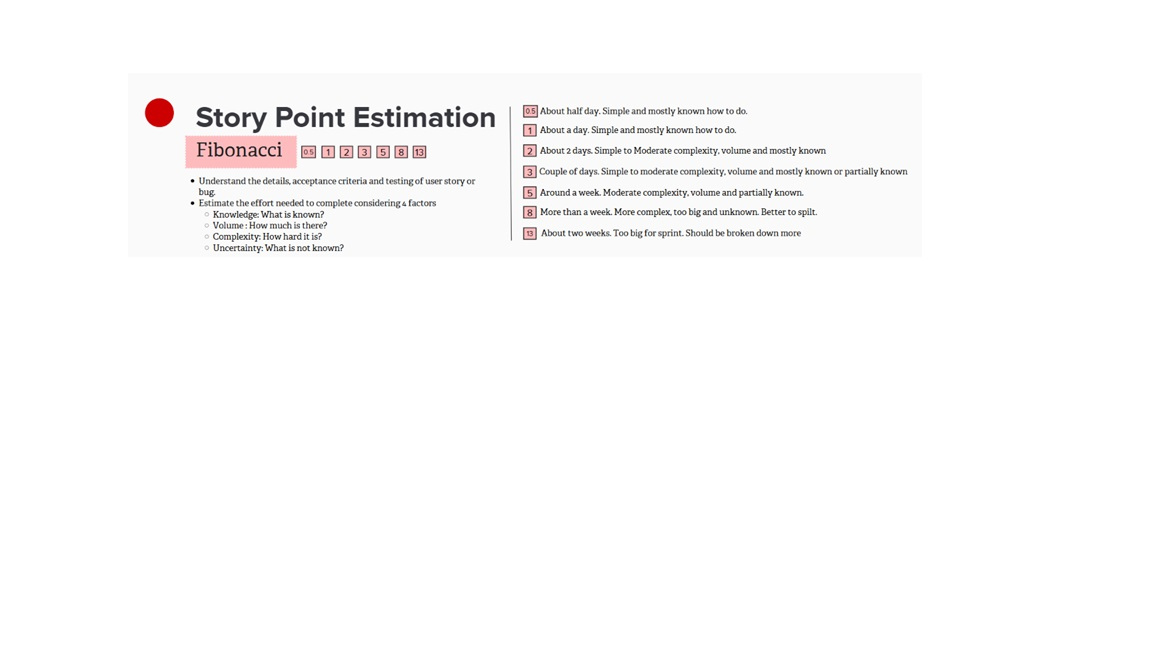
\includegraphics[width=0.7\textwidth]{figures/example.jpg}
\caption{Xxxxx}
\label{fig:figura1}
\textit{Nota}. Adaptado de Virus VIH [Fotografía], por Consejo Superior de Investigaciones Científicas, 2011, Flickr (flic.kr/p/aronSf). CC BY 2.0.
\end{figure}
\clearpage

% capitulo2.tex
\chapter{Marco Teórico y Revisión de Literatura}

\section{Xxxxxxxxxx xxxxxx xxxxxxx xxxx}

Xxxxxxxxxxxxxxxxxxxxxxxxxxxxxxxxxxxxxxxxxxxxxxxxxxxxxxxxxxxxxxxxxxxxxxxxxxxxxxxxxxxxxxxxxxxxxxxxxxxxxxxxxxxxxxxxxxxxxxxxxxxxxxxxxxxxxxxxxxxxxxxxxxxxxxxxxxxxxxxxxxxxxxxxxxxxxxxxxxxxxxxxxxxxxxxxxxxxxxxxxxxxxxxxxxxxxxxxxxxxxxxxxxxxxxxxxxxxxxxxxxxxxxxxxxxxxxxxxxxxxxxxxxxxxxxxxxxxxxxxxxxxxxxxxxxxxxxxxxxxxxxxxxxxxxxxxxxxxxxxxxxxxxxxxxxxxxxxxxxxxxxxxxxxxxxxxxxxxxxxxxxxxxxxxxxxxxxxxxxxxxxxxxxxxx.

Xxxxxxxxxxxxxxxxxxxxxxxxxxxxxxxxxxxxxxxxxxxxxxxxxxxxxxxxxxxxxxxxxxxxxxxxxxxxxxxxxxxxxxxxxxxxxxxxxxxxxxxxxxxxxxxxxxxxxxxxxxxxxxxxxxxxxxxxxxxxxxxxxxxxxxxxxxxx.

\section{Xxxxxxx xxxxxx xxxxxxxxx xxxxxxx}

Xxxxxxxxxxxxxxxxxxxxxxxxxxxxxxxxxxxxxxxxxxxxxxxxxxxxxxxxxxxxxxxxxxxxxxxxxxxxxxxxxxxxxxxxxxxxxxxxxxxxxxxxxxxxxxxxxxxxxxxxxxxxxxxxxxxxxxxxxxxxxxxxxxxxxxxxxxxxxxxxxxxxxxxxxxxxxxxxxxxxxxxxxxxxxxxxxxxxxxxxxxxxxxxxxxxxxxxxxxxxxxxxxxxxxxxxxxxxxxxxxxxxxxxxxxxxxxxxxxxxxxxxxxxxxxxxxx.

Xxxxxxxxxxxxxxxxxxxxxxxxxxxxxxxxxxxxxxxxxxxxxxxxxxxxxxxxxxxxxxxxxxxxxxxxxxxxxxxxxxxxxxxxxxxxxxxxxxxxxxxxxxxxxxxxxxxxxxxxxxxxxxxxxxxxxxxxxxxxxxxxxxxxxxxxxxxxxxxxxxxxxxxxxxxxxxxxxxxxxxxxxxxxxxxxxxxxxxxxxxxxxxxxxxxxxxxxxxxxxxxxxxxxxxxxxxxxxxxxxxxxxxxxxxxxxxxxxxxxxxxxxxxxxxxxxxxxxxxxxxxxxxxxxxxxxxxxxxxxxxxxxxxxxxxxxxxxxxxxxxxxxxxxxxxxxxxxxxxxxxxxxxxxxxxxxxxxxxxxxxxxxxxxxxxxxxxxxxxxxxxxxxxxxxxxxxxxxxxxxxxxxxxxxxxxxxxxxxxxxxxxxxxxxxxxxxxxxxxxxxxxxxxxxxxxx.

Xxxxxxxxxxxxxxxxxxxxxxxxxxxxxxxxxxxxxxxxxxxxxxxxxxxxxxxxxxxxxxxxxxxxxxxxxxxxxxxxxxxxxxxxxxxxxxxxxxxxxxxxxxxxxxxxxxxxxxxxxxxxxxxxxxxxxxxxxxxxxxxxxxxxxxxxxxxxxxxxxxxxxxxxxxxxxxxxxxxxxxxxxxxxxxxxxxxxxxxxxxxxxxxxxxxxxxxxxxxxxxxxxxxxxxxxxxxxxxx
\clearpage

% capitulo3.tex
\chapter{Nombre del capítulo}

\section{Xxxxxxxxx}

Xxxxxxxxxxxxxxxxxxxxxxxxxxxxxxxxxxxxxxxxxxxxxxxxxxxxxxxxxxxxxxxxxxxxxxxxxxxxxxxxxxxxxxxxxxxxxxxxxxxxxxxxxxxxxxxxxxxxxxxxxxxxxxxxxxxxxxxxxxxxxxxxxxxxxxxxxxxxxxxxxxxxxxxxxxxxxxxxxxxxxxxxxxxxxxxxxxxxxxxxxxxxxxxxxxxxxxxxxxxxxxxxxxxxxxxxxxxxxxxxxxxxxxxxxxxxxxxxxxxxxxxxxxxxxxxxxxxxxxxxxxxxxxxxxxxxxxxxxxxxxxxxxxxxxxxxxxxxxxxxxxxxxxxxxxxxxxxxxxxxxxxxxxxxxxxxxxxxxxxxxxxxxxxxxxxxxxxxxxxxxxxxxxxxxxxxxxxxxxxxxxxxxxxxxxxxxxxxxxxxxxxxxxxxxxxxxxxxxxxxxxxxxxxxxxxxxxxxxxxxxxxxx.

Xxxxxxxxxxxxxxxxxxxxxxxxxxxxxxxxxxxxxxxxxxxxxxxxxxxxxxxxxxxxxxxxxxxxxxxxxxxxxxxxxxxxxxxxxxxxxxxxxxxxxxxxxxxxxxxxxxxxxxxxxxxxxxxxxxxxxxxxxxxxxxxxxxxxxxxxxxxxxxxxxxxxxxxxxxxxxxxxxxxxxxxxxxxxxxxxxxxxxxxxxxxxxxxxxxxxxxxxxxxxxxxxxxxxxxxxxxxxxxxxxxxxxxxxxxxxxxxxxxxxxxxxxxxxxxxxxxxxxxxxxxxxxxxxxxxxxxxxxxxxxxxxxxxxxxxxxxxxxxxxxxxxxxxxxxxxxxxxxxxxxxxxxxxxxxxxxxxxxxxxxxxxxxxxxxxxxxxxxxxxxxxxxxxxxxxxxxxxxxxxxxxxxxxxxxxxxxxxxxxxxxxxxxxxxxxxxxxxxxxxxxxxxxxxxxxxxxxxxxxxxxxxxx.

\section{Xxxxxxxxx xxxxxxx xxxxxx xxxxxx xxxxxxx}

Xxxxxxxxxxxxxxxxxxxxxxxxxxxxxxxxxxxxxxxxxxxxxxxxxxxxxxxxxxxxxxxxxxxxxxxxxxxxxxxxxxxxxxxxxxxxxxxxxxxxxxxxxxxxxxxxxxxxxxxxxxxxxxxxxxxxxxxxxxxxxxxxxxxxxxxxxxxxxxxxxxxxxxxxxxxxxxxxxxxxxxxxxxxxxxxxxxxxxxxxxxxxxxxxxxxxxxxxxxxxxxxxxxxxxxxxxxxxxxxxxxxxxxxxxxxxxxxxxxxxxxxxxxxxxxxxxxxxxxxxxxxxxxxxxxxxxxxxxxxxxxxxxxxxxxxxxxxxxxxxxxxxxxxxxxxxxxxxxxxxxxxxxxxxxxxxxxxxxxxxxxxxxxxxxxxxxxxxxxxxxxxxxxxxxxxxxxxxxxxxxxxxxxxxxxxxxxxxxxxxxxxxxxxxxxxxxxxxxxxxxxxxxxxxxxxxxxxxxxxxxxxxxx.

Xxxxxxxxxxxxxxxxxxxxxxxxxxxxxxxxxxxxxxxxxxxxxxxxxxxxxxxxxxxxxxxxxxxxxxxxxxxxxxxxxxxxxxxxxxxxxxxxxxxxxxxxxxxxxxxxxxxxxxxxxxxxxxxxxxxxxxxxxxxxxxxxxxxxxxxxxxxxxxxxxxxxxxxxxxxxxxxxxxxxxxxxxxxxxxxxxxxxxxxxxxxxxxxxxxxxxxxxxxxxxxxxxxxxxxxxxxxxxxxxxxxxxxxxxxxxxxxxxxxxxxxxxxxxxxxxxxxxxxxxxxxxxxxxxxxxxxxxxxxxxxxxxxxxxxxxxxxxxxxxxxxxxxxxxxxxxxxxxxxxxxxxxxxxxxxxxxxxxxxxxxxxxxxxxxxxxxxxxxxxxxxxxxxx.
\clearpage

% Conclusiones
% conclusiones.tex
\chapter*{Conclusiones}
\addcontentsline{toc}{chapter}{Conclusiones}

Se redactan los puntos más sobresalientes, debilidades o fortalezas del proyecto o investigación, observados o descubiertos durante la ejecución del Trabajo de Integración Curricular, se recomienda redactar por cada conclusión, una recomendación.
\clearpage

% Recomendaciones
% recomendaciones.tex
\chapter*{Recomendaciones}
\addcontentsline{toc}{chapter}{Recomendaciones}

En esta parte debes sugerir temas para futuras investigaciones y puedan aportar a la academia.

Xxxxxxxxxxxxxxxxxxxxxxxxxxxxxxxxxxxxxxxxxxxxxxxxxxxxxxxxxxxxxxxxxxxxxxxxxxxxxxxxxxxxxxxxxxxxxxxxxxxxxxxxxxxxxxxxxxxxxxxxxxxxxxxxxxxxxxxxxxxxxxxxxxxxxxxxxxxxxxxxxxxxxxxxxxxxxxxxxxxxxxxxxxxxxxxxxxxxxxxxxxxxxxxxxxxxxxxxxxxxxxxxxxxxxxxxxxxxxxxxxxxxxxxxxxxxxxxxxxxxxxxxxxxxxxxxxxxxxxxxxxxxxxxxxxxxxxxxxxxxxxxxxxxxxxxxxxxxxxxxxxxxxxxxxxxxxxxxxxxxxxxxxxxxxxxxxxxxxxxxxxxxxxxxxxxxxxxxxxxxxxxxxxxxxxxxxxxxxxxxxxxxxxxxxxxxxxxxxxxxxxxxxxxxxxxxxxxxxxxxxxxxxxxxxxxxxxxxxxxxxxxxxx.

Xxxxxxxxxxxxxxxxxxxxxxxxxxxxxxxxxxxxxxxxxxxxxxxxxxxxxxxxxxxxxxxxxxxxxxxxxxxxxxxxxxxxxxxxxxxxxxxxxxxxxxxxxxxxxxxxxxxxxxxxxxxxxxxxxxxxxxxxxxxxxxxxxxxxxxxxxxxxxxxxxxxxxxxxxxxxxxxxxxxxxxxxxxxxxxxxxxxxxxxxxxxxxxxxxxxxxxxxxxxxxxxxxxxxxxxxxxxxxxxxxxxxxxxxxxxxxxxxxxxxxxxxxxxxxxxxxxxxxxxxxxxxxxxxxxxxxxxxxxxxxxxxxxxxxxxxxxxxxxxxxxxxxxxxxxxxxxxxxxxxxxxxxxxxxxxxxxxxxxxxxxxxxxxxxxxxxxxxxxxxxxxxxxxx.
\clearpage

% Referencias
\printbibliography[heading=bibintoc,title={Referencias}]
\clearpage


\end{document}